\documentclass{article}
\usepackage{tikz}
\usepackage{tikz-uml}

\begin{document}

\section{Sintaxis}
Cada figura se abre con \verb|\begin{tikzpicture}| y cada clase se declara
con \verb+\umlclass{Nombre}{atributos}{métodos}+ dentro de ella. Por ejemplo:

\begin{verbatim}
\begin{tikzpicture}
  \begin{umlpackage}{ejemplo}
    \umlclass{Ejemplo}{- x : int}{+ f() : void}  % comentario
  \end{umlpackage}
  \umlrelationship{Ejemplo}{Ejemplo}
\end{tikzpicture}
\end{verbatim}

Más del 90\% de las figuras de este documento son diagramas de clases.
% Este inicio de entorno se ignora por estar en un comentario \begin{verbatim}

\section{Diagramas}
% Figura 1: un esquema que no es un diagrama de clases
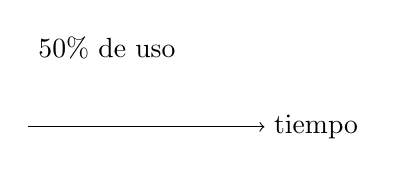
\begin{tikzpicture}
   \draw[->] (0,0) -- (3,0) node[right] {tiempo};
   \node at (1,1) {50\% de uso};
\end{tikzpicture}

% Este fin de entorno se ignora por estar en un comentario \end{document}


% Figura 2: diagrama de clases
\begin{tikzpicture}
\begin{umlpackage}{banco}
   \umlclass[type=interface]
      {Auditable}{}{
      + auditar() : void
   }
   \umlclass[x=6]{Cuenta}{
      \# saldo : float \\
      - comision : float = 1.5\% \\ - titular : string \\
      - numCuentas : int
   }{
      + ingresar(c : float) : void \\
      + consultar(campos : \{string\}) : float
   }
   \umlclass[x=6, y=-5]{CuentaAhorro}{ - interes : float }{
      + liquidar() : void
   }
\end{umlpackage}
\umlclass[x=12]{Registro}{ entradas : int }{}

\umlrelationship[type=implementation]{Cuenta}{Auditable}
\umlrelationship[type=inheritance, geometry=|-]{CuentaAhorro}{Cuenta}
% \umlrelationship[type=association]{Registro}{Cuenta}
\end{tikzpicture}

\end{document}
